\documentclass[aspectratio=169]{beamer}

\usepackage[utf8]{inputenc}
\usecolortheme{beaver}
\usepackage{caption}
\usepackage{subcaption}
\usepackage{mathtools}
\usepackage{todonotes}
\usepackage{amsmath}
\usepackage{bm}
\usepackage{listings}
\usepackage{ragged2e}
\usepackage{titlecaps}
\usepackage{fancyvrb}
\usepackage[export]{adjustbox}
\def\ci{\perp\!\!\!\!\!\perp}

\newtheorem{proposition}{Proposition}
\Addlcwords{for a is but and with of in as the etc on to if}

\newcommand{\stackwords}[4]{\begin{tabular}[t]{@{}l@{}l@{}l@{}}#1\\#2\\#3\\#4\end{tabular}}

\setbeamertemplate{section in toc}{\inserttocsectionnumber.~\inserttocsection}
\usetheme{Boadilla}
\makeatletter
\setbeamertemplate{footline}{%
    \leavevmode%
    \hbox{%
        \begin{beamercolorbox}[wd=.3\paperwidth,ht=2.25ex,dp=1ex,center]{author in head/foot}%
            \usebeamerfont{author in head/foot}\insertshortauthor\expandafter\beamer@ifempty\expandafter{\beamer@shortinstitute}{}{~~(\insertshortinstitute)}
        \end{beamercolorbox}%
        \begin{beamercolorbox}[wd=.55\paperwidth,ht=2.25ex,dp=1ex,center]{title in head/foot}%
            \usebeamerfont{title in head/foot}\insertshorttitle
        \end{beamercolorbox}%
        \begin{beamercolorbox}[wd=.15\paperwidth,ht=2.25ex,dp=1ex,right]{date in head/foot}%
            \usebeamerfont{date in head/foot}\insertshortdate{}\hspace*{2em}
            \insertframenumber{} / \inserttotalframenumber\hspace*{2ex} 
        \end{beamercolorbox}}%
        \vskip0pt%
    }
\makeatother

\begin{document}

\title{Testing and Estimation in Causal Models}
\subtitle{Addressing Mixed and Missing Data Challenges}
\author{Ankur Ankan}
\institute[]{Radboud University, The Netherlands}
\date{}

\maketitle

\begin{frame}{Causal Inference}
	\center{\Large{Many questions in science are causal}}
	\vspace{0.5em}
	\only<2>{
	\begin{figure}
		\begin{subfigure}{0.3 \textwidth}
			\includegraphics[scale=0.1, valign=m]{imgs/vaccine.png}
		\end{subfigure}
		\qquad\tikz[baseline=-\baselineskip]\draw[ultra thick,->] (-1,0) -- ++ (1,0);\qquad	
		\begin{subfigure}{0.3 \textwidth}
			\includegraphics[scale=0.1, valign=m]{imgs/infectious.png}
		\end{subfigure}
	\end{figure}

	\vspace{0.5em}
	Epidemiology: Does vaccination reduce the spread of infectious disease?
	}
	\only<3>{
	\begin{figure}
		\begin{subfigure}{0.35 \textwidth}
			\includegraphics[scale=0.1, valign=m]{imgs/video_game.png}
		\end{subfigure}
		\qquad\tikz[baseline=-\baselineskip]\draw[ultra thick,->] (0,0) -- ++ (1,0);\qquad	
		\begin{subfigure}{0.35 \textwidth}
			\includegraphics[scale=0.1, valign=m]{imgs/fight.png}
		\end{subfigure}
	\end{figure}
	Social Sciences: Does exposure to violent video games increase aggressive behavior in children?
	}
	\only<4>{
	\begin{figure}
		\begin{subfigure}{0.35 \textwidth}
			\includegraphics[scale=0.1, valign=m]{imgs/deforestation.png}
		\end{subfigure}
		\qquad\tikz[baseline=-\baselineskip]\draw[ultra thick,->] (0,0) -- ++ (1,0);\qquad	
		\begin{subfigure}{0.35 \textwidth}
			\includegraphics[scale=0.1, valign=m]{imgs/climate_change.png}
		\end{subfigure}
	\end{figure}

	Environmental Science: Does deforestation contribute to climate change and loss of biodiversity?
	}
\end{frame}

\begin{frame}{Causal Inference}
	\center{\large{\textbf{Goal:} Understand how an \stackwords{\textbf{intervention}}{vaccination}{video games}{deforestation} influences an \stackwords{\textbf{outcome}.}{infection spread}{aggressive behavior}{climate change}}}

	\vspace{2em}

	\begin{itemize}
		\item \textbf{Understand Causal Relationships: }
			\begin{itemize}
				\item Whether an intervention impacts the outcome.
				\item Examine if the effect is direct, or indirect, occurring through intermediary factors.
			\end{itemize}
		\item \textbf{Quantify Causal Relationships: }
			\begin{itemize}
				\item Measure the magnitude of the intervention's impact.
				\item For example, if we increase deforestation by 2x, how much impact would it have on climate change.
			\end{itemize}
	\end{itemize}
\end{frame}

\begin{frame}{Randomized Controlled Trial}	
	\center{Best way to answer these causal questions is using \textbf{Randomized Controlled Trials}.}
	\todo[inline]{Insert a figure here}
\end{frame}

\begin{frame}{Randomized Controlled Trial}
	\center{However, randomized controlled trials are \textbf{not always feasible.}}
	
	\vspace{2em}

	\begin{itemize}[<+->]
		\item \textbf{Unethical: } To study the effect of smoking on lung cancer, we can not ask non-smokers to start smoking.
		\item \textbf{Difficult to control exposures:} To study the effects of deforestation on climate, we can not create a clone of earth.
		\item \textbf{Cost:} Assessing the effect of education on income would require decades of tracking individuals.
	\end{itemize}

	\vspace{2em}

\only<4>{
\center{Can we answer these questions using data that we already have?}}
\end{frame}

\begin{frame}{Causal Graphs}
	\center{Yes, but we need to understand the causal mechanism.}

	\todo[inline]{Show an example of a DAG. Show causal paths, and causal effects.}

	\todo[inline]{Highlight what the two tasks outlined before mean in terms of Causal Graphs}
	\begin{itemize}
		\item Causal relationship $ \implies $ causal paths.
		\item Quantification $ \implies $ Strength of these edges.
	\end{itemize}
\end{frame}

\begin{frame}{Mixed and Missing Data}
	\center{I have focused on improving these methods for mixed and missing data.}

	\textbf{Mixed Data:}
		\begin{enumerate}
			\item Numerical:
			\item Categorical:
			\item Ordinal:
		\end{enumerate}

	\textbf{Missing Data:} Not all variables can be measured. For example climate change.
\end{frame}

\begin{frame}{Constructing Causal Graphs}
\center{How do we construct these causal graphs?}

\center{Usually done manually based on knowledge}

\center{Important to test whether our causal graph is correct.}

\begin{figure}
	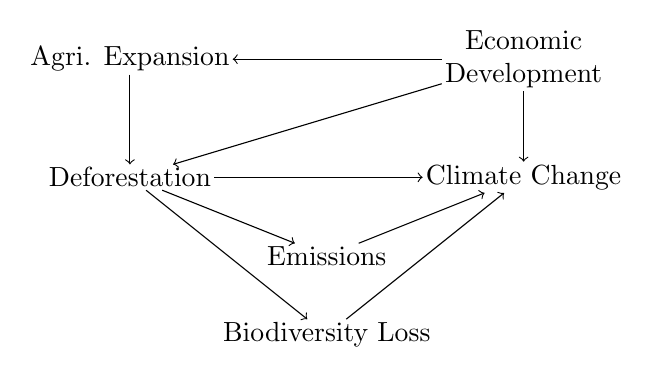
\begin{tikzpicture}
		\begin{scope}[scale=1]
		\tikzstyle{every node}=[align=center, inner sep=1pt]
				\node (D) at (0, 0) {Deforestation};
				\node (CC) at (5, 0) {Climate Change};
				\node (E) at (2.5, -1) {Emissions};
				\node (BL) at (2.5, -2) {Biodiversity Loss};
				\node (ED) at (5, 1.5) {Economic \\ Development};
				\node (AE) at (0, 1.5) {Agri. Expansion};
			
				\draw[->]  (D) -- (CC);
				\draw[->]  (D) -- (E);
				\draw[->]  (D) -- (BL);
				\draw[->]  (E) -- (CC);
				\draw[->]  (BL) -- (CC);
				\draw[->]  (ED) -- (D);
				\draw[->]  (ED) -- (AE);
				\draw[->]  (AE) -- (D);
				\draw[->]  (ED) -- (CC);
		\end{scope}
	\end{tikzpicture}
\end{figure}
	
\end{frame}

\begin{frame}{Testing Casual Graphs}

	Graph $ \implies $ Independence statements.
	Independence means 

	Selecting the correct conditional independence test depends on a lot of factors.

	In one of the chapters, we presented a practical guide for researchers trying to apply these methods in their research on how to carry out this testing.
\end{frame}

\begin{frame}{Conditional Independence Tests}
	Model testing relies on these statistical Conditional independence tests.
	Conditional Independence tests can also be used for constructing these graphs
	automatically.

	Hence, important that these tests are accurate.
\end{frame}

\begin{frame}{Chapter 3: CI test for testing and constructing graph}
	The model testing utilizes conditional independence tests.

	In Chapter 3, we propose a novel test for mixed data.
\end{frame}

\begin{frame}{Causal Effect Estimation}
	Some of the variables are unobserved.
	Impossible to estimate the effect.
	Trick: Use an observed child of the variable to estimate it by fixing one of the
	variables.
\end{frame}

\begin{frame}{Software}
	To make it easy for these methods to use, we have a software package.
\end{frame}

\begin{frame}{Future research}
\end{frame}

\begin{frame}
	\Huge{Thank you}
\end{frame}

\end{document}
